% ----------------------------------------------------------------------------------------\
% ---------------------------------------------------------------------------------------\
% --------------------------------------------------------------------------------------\
\section{Desarrollo}
% ----------------------------------------------------------------------------------------\
% ---------------------------------------------------------------------------------------\
% --------------------------------------------------------------------------------------\
% Explicación de las implementaciones, diagrama de flujo, ideas, comentarios, investigación, etc
% ----------------------------------------------------------------------------------------\
% ---------------------------------------------------------------------------------------\
\subsection{Implementación básica del Juego de la Vida}
% ----------------------------------------------------------------------------------------\
% ---------------------------------------------------------------------------------------\
El Juego de la vida es un autómata celular, es decir es un modelo matemático llevado de manera computacional para observar de manera dinámica cómo evoluciona en el tiempo. Creado por John Horton Conway en 1969 que consiste en una cuadrícula donde se marcan o desmarcan siendo pintados por un color, representando células y reflejando si esta se encuentra viva o muerta.


Iniciado el juego son las reglas las que determinan como acaba. El objetivo es crear un sistema que simulase la vida y su naturaleza. La manera en que se logra es con el nacimiento y supervivencia de estos seres binarios digitales donde depende del número de vecinos que estén a su vez vivos o muertos. Por lo que es posible observar patrones complejos e impredecibles gracias a unas sencillas reglas. Siendo utilizado como un modelo de simulación para estudiar fenómenos biológicos, evolutivos o físicos.

\begin{figure}[H]
    \centering
    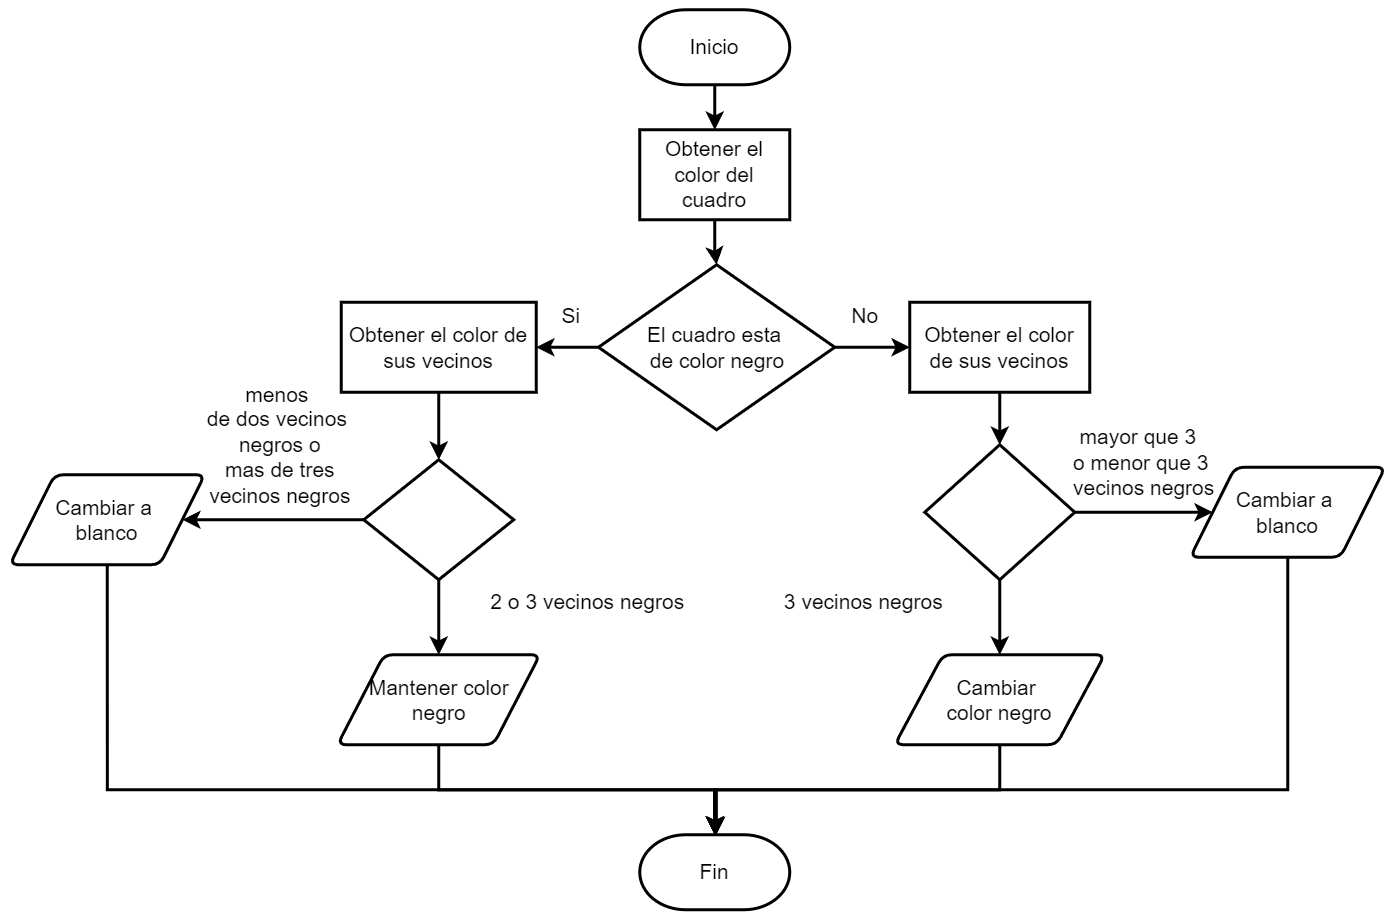
\includegraphics[width=0.9\linewidth]{IMA/DiagramaFlujoJuegoLaVida.png} 
    \caption{Diagrama de flujo del Juego de la Vida} 
\end{figure}

En el diagrama se puede observar las reglas que se siguen para determinar si una célula vive o muere.
En este caso las condicionales del diagrama reflejan la sobrepoblación, la soledad , la reproducción y la supervivencia de las células.
Por lo que solo faltaria implementar el código en Python para poder visualizar el juego de la vida.


% ----------------------------------------------------------------------------------------\
% ---------------------------------------------------------------------------------------\
\subsection{Introducción a los Algoritmos Genéticos}
% ----------------------------------------------------------------------------------------\
% ---------------------------------------------------------------------------------------\




% ----------------------------------------------------------------------------------------\
% ---------------------------------------------------------------------------------------\
\subsection{Implementación de Algoritmos Genéticos en el Juego de la Vida}
% ----------------------------------------------------------------------------------------\
% ---------------------------------------------------------------------------------------\

Recordemos las reglas iniciales del juego:
\begin{enumerate}
    \item Si una célula está viva y tiene dos o tres vecinas vivas, sobrevive.
    \item Si una célula está muerta y tiene tres vecinas vivas, nace.
    \item Si una célula está viva y tiene más de tres vecinas vivas, muere.
    
    La disposición o patrón inicial de células se llama \textit{semilla}. La siguiente 
    generación nace de aplicar las reglas del juego a todas las células de manera 
    simultánea. Este proceso se puede ejecutar de manera indefinida.
\end{enumerate}

% ----------------------------------------------------------------------------------------\
\subsubsection*{Modificación de las Reglas}
% ----------------------------------------------------------------------------------------\

Para modificar la simulación del Juego por los cromosomas de una población podemos crear
una \textbf{representación cromosómica:} donde cada cromosoma será una cadena binaria 
donde cada bit representa el estado de una célula en el tablero (vivo o muerto).\\ 

Así las nuevas reglas para el \textit{Juego de la Vida} que estamos proponiendo es para 
buscar crear más vida con menos generaciones, las células  podrán vivir con más vecinos 
si se alcanza un cierto número de cromosomas en la población:

\begin{itemize}
    \item Nacimientos: Una célula muerta con exactamente tres vecinos vivos se convierte 
    en una célula viva.
    \item Muerte uno: Una célula viva con uno o menos vecinos vivos muere.
    \item Muerte dos: Una célula viva con más de tres vecinos vivos muere, a menos que se 
    cumpla la condición especial.
    \item Condición Especial de Supervivencia: Si la población de cromosomas alcanza o 
    supera un $n$ especifica, las células vivas pueden soportar hasta cuatro 
    vecinos vivos sin morir.
    \item Supervivencia Normal: Si no se cumple la condición especial, una célula viva con 
    dos o tres vecinos vivos sobrevive.
    \item Muerte tres: Si en $n$ generaciones no se alcanza el objetivo el juego termina.
\end{itemize}

El objetivo que queremos lograr con este cambio es encontrar un conjunto de células más eficiente
en el menor tiempo de generaciones, para este caso definiremos que sea cumplido tras un 
70 porciento del total de generaciones (aproximadamente 160 generaciones), es decir, buscamos 
las células que se mantengan como población estable y amplia cumpliendo los criterios de aptitud.

% ----------------------------------------------------------------------------------------\
\subsubsection*{Pasos del algoritmo}
% ----------------------------------------------------------------------------------------\

\begin{itemize}
    \item Inicialización de la Población: Generamos una población inicial de cromosomas de 
    manera aleatoria
    \item Evaluación de la Aptitud: astronaves
    \item Selección: Utilizamos un método de selección por torneo
    \item Reproducción: Cruzamiento en dos puntos, en el que se intercambian los genes que 
    aparecen en el intervalo de genes delimitados por dos puntos.
    \item Mutación: Cambiar aleatoriamente el estado de algunas células
    \item Remplazo: Una vez realizada la mutación y aplicar una evaluación fitness (más 
    tranquila que la evaluación de la aptitud) se hace el remplazo
\end{itemize}


% ----------------------------------------------------------------------------------------\
\subsubsection*{Inicialización de la Población}
% ----------------------------------------------------------------------------------------\

Cada célula en el tablero de $n \times n$ tiene ocho vecinos, que incluyen las celdas 
adyacentes horizontal, vertical y diagonalmente. Al comienzo del juego, la población inicial 
se genera aleatoriamente, cada cromosoma es una secuencia binaria que representa un estado 
completo del tablero, con 1s para las células vivas y 0s para las muertas.

\subsubsection*{Función fitness}

Para definir la función fitness necesitamos saber que existen patrones básicos dentro del 
juego y estos son configuraciones de los vecinos para las células que determinan un 
comportamiento concreto como patrones estáticos que no hay nacimientos ni fallecimientos,
y nunca cambian, patrones recurrentes o \textit{osciladores} que evolucionan a través de 
diversos estados pero vuelven a su forma inicial y patrones que se trasladan por el tablero
llamados \textit{spaceships}.\\ 

Las astronaves \cite{spaceships} son patrones que se caracterizan por desplazarse a través 
del tablero a lo largo del tiempo, bien sea de forma diagonal o de forma horizontal o 
vertical. La velocidad de desplazamiento es variable, dependiendo del patrón que se trate.
y esta capacidad para moverse eficientemente es un indicador de su robustez y estabilidad 
dentro del juego\\ 

\noindent La fórmula de velocidad para las \textit{spaceships}:

\begin{equation*}
    v = \frac{max(|x|,|y|)}{n} \times c
\end{equation*}

\begin{itemize}
    \item[] ($v$) es la velocidad de la astronave.
    \item[] ($x$) y ($y$) son los desplazamientos en dos dimensiones (horizontal y vertical).
    \item[] ($n$) es el número de generaciones que tarda la astronave en desplazarse.
    \item[] ($c$) es una constante análoga a la velocidad de la luz, que en este contexto se 
    puede considerar como 1 celda por generación.
\end{itemize}

Esta fórmula es útil para medir la eficiencia con la que un patrón se desplaza a través del 
tablero. Los patrones que se mueven más rápido (mayor valor de ($v$)) serían considerados 
más \textit{aptos} mientras que con velocidades más bajas nos dice que esos patrones son menos
eficientes (lentos) o que mueren rápidamente, de manera que calificaran con aptitud menor.\\    


Entonces estamos considerando la distancia máxima recorrida en cualquier dirección y el 
número de generaciones necesarias para dicho desplazamiento, la ventaja de usar la velocidad
para hacer la evaluación es que favorece patrones que pueden sobrevivir y moverse a lo largo de 
las generaciones, como si fuera una evolución natural sin embargo se añadió otro criterio el 
cual consiste en sumar puntos si es que los patrones no chocan demasiado con los bordes, ya que 
células vivas en bordes podrían tener menos vecinos para sobrevivir. 